%% title: Head Chains and Do-Support
%% category: theories

\begin{abstract}
English auxiliaries come in two kinds: those that move to C and those that need \textit{do}. This chapter argues that the difference lies not in the auxiliaries themselves but in where the head chain they belong to is pronounced.
\end{abstract}
\label{ch:chains}

\section{Four kinds of \textit{have}}\label{sec:have}

Possessive \textit{have} is unusual among English verbs: some varieties let it invert, as in \Next[c], while others require \textit{do}-support, as in \Next[d].

\pex \dref{fourhaves}
 \a \textbf{Have} I eaten enough jam? \hfill(perfect \textit{have})
    \a Did Jim \textbf{have} his car break down? \hfill(affective \textit{have})
    \a \textbf{Have} you any jam? \hfill (possessive \textit{have} in NBrE\footnote{AmE refers to most American Englishes; NBrE refers to some northern British Englishes.})
    \a Do you \textbf{have} any jam? \hfill (possessive \textit{have} in AmE) \xe

Perfect \textit{have} in \Last[a] behaves like a true auxiliary, while affective \textit{have} in \Last[b] never inverts. \citet{bjorkman2011} treats auxiliaries as a last resort for stranded inflection; the question here is why possessive \textit{have} sits on both sides of the line.

\section{Inversion past an applicative}\label{sec:appl}

In some Scots varieties, possessive \textit{have} can be followed by an applicative phrase. When it is, inversion is impossible: \textit{have} cannot cross the applicative head to reach C, and \textit{do} is inserted instead.

\ex \dref{scotsappldiagram} \Lb{CP} \rnode{do}{do} \Lb{TP} \rnode{you}{you} \dots \rnode{have}{have} \dots \Lb{ApplP} \rnode{appl}{\textsc{\textbf{Appl}}} that charger with you ? ] ] ]
    \ncbar[angle=-90,arm=9pt]{->}{have}{do}
    \ncput*{\rnode{xm}{\xm}} \xe

The blocked movement in \gref{scotsappldiagram} contrasts with \LLast[c], where nothing intervenes and possessive \textit{have} inverts freely.\comment{Check whether the Appl effect survives with pronominal objects.}

\section{Head chains}\label{sec:chains}

In interrogatives, C, T and the verbal category Vc form a single chain whose morphology is spelled out in C, as \textit{did}; the lexical verb heads a chain of its own \Next[a]. With an auxiliary, the chain is pronounced lower, between T and Aux \Next[b].

{\singlespacing
\begin{multicols}{2}
\ex a. Interrogatives\\
\\
    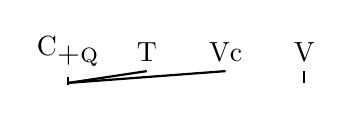
\begin{tikzpicture}[
          dep/.style={line width=0.8pt}
        ]
        \node (C1) at (0,0) {C$_{\textsc{+q}}$};
        \node (T1) at (1,0) {T};
        \node (O1) at (2,0) {Vc};
        \node (V1) at (3,0) {V};
        \draw[dep] (C1.south) -- ++ (0,-0.11);
        \draw[dep] (T1.south) -- ++(-1,-0.15);
        \draw[dep] (O1.south) -- ++ (-2,-0.15);
        \draw[dep] (V1.south) -- ++(0,-0.15);
    \end{tikzpicture} \\
    \textit{\phantom{a}\textbf{did} you \phantom{aaaaaaaaaa} \textbf{eat}?}
\xe
\columnbreak

\hspace*{-7mm} b. Auxiliaries\\
\\
    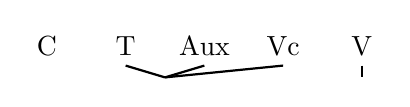
\begin{tikzpicture}[
        dep/.style={line width=0.8pt}
        ]
        \node (C1) at (0,0) {C};
        \node (T1) at (1,0) {T};
        \node (P1) at (2,0) {Aux};
        \node (O1) at (3,0) {Vc};
        \node (V1) at (4,0) {V};
        \draw[dep] (T1.south) -- ++(0.5,-0.15);
        \draw[dep] (P1.south) -- ++(-0.5,-0.15);
        \draw[dep] (O1.south) -- ++ (-1.5,-0.15);
        \draw[dep] (V1.south) -- ++ (0,-0.15);
    \end{tikzpicture}\\
    \textit{\phantom{a} you \phantom{a} \textbf{should} \phantom{aaaaaaaaaa} \textbf{eat}.}
\end{multicols}}

The same diagrams can be written with the \texttt{\textbackslash headchain} shorthand, which works out the spacing itself. With sentential negation, T and Vc cannot form a chain across Neg, so T is pronounced on its own as \textit{did} \Next[b].

\pex \dref{chainshorthand}
  \a \headchain{[*C$_{\textsc{+q}}$ T Vc]{did} (you) [V]{eat}}
  \a \headchain{C (you) [T]{did} [Neg]{not} [Vc *V]{eat}}
\xe

\section{Why chains are pronounced where they are}\label{sec:causality}

Whether a head is pronounced depends on two decisions, taken in order \Next.

\ex \hspace*{-10mm}
\begin{forest}for tree={s sep=10pt}
    [A given head Z{[*]}
        [assigned overt \\ morphology at insertion, draw]
        [not assigned overt \\ morphology at insertion
            [placed in a head chain \\ with overt morphology, draw]
            [not placed in a head chain \\ with overt morphology, draw]]]
\end{forest} \xe

The second branch is where \textit{do}-support lives. A head Z bearing an unvalued [*] feature that receives no morphology of its own must be rescued by a chain; if no chain is available, as in \gref{do-support}, a dummy is inserted.

\begin{multicols}{2}
\ex \dref{do-support}
    \begin{forest}
        [XP
            [X]
            [YP
                [Y{[\#]} \\ /\dots/]
                [\dots \\ ZP
                    [Z{[*]}\\ /\nothing/]]]]
        \begin{scope}[shift={(-2em,-4.7em)}]
        \draw (0.5,0.5) edge[bend left] (2.2,1.2);
        \end{scope}
    \end{forest}
\xe
\columnbreak
\exdisplay\noexno
    \begin{tikzpicture}
        [>=Stealth, thick]
        \node[draw, circle] (a) at (0,3.25) {X};
        \node[draw, circle] (b) at (0,1.4) {Y};
        \node[draw, circle] (d) at (0,0) {Z};
        \draw[->, gray, dashed, thick] (0,2.4) -- (d.north);
        \draw[->] (0,2.4) -- (b);
        % \node[draw, circle] (b) at (0,2) {Y};
        % \draw[->] (b) -- (0,1);
        \draw[pattern=north east lines] (-2,0.7) rectangle (2,1);
        \node at (2.45,0.85) {[\#]};
    \end{tikzpicture}
\xe
\end{multicols}

The picture on the right is the physical analogy: the [\#] layer is a barrier that the dependency from X can reach but not cross, so Z is never reached.
